\pattern{Observer}
\begin{summary}
    The {\bf Observer} pattern is characterized by a subject and many observers
    which are ``observing'' the subject and reacting to change. The subject
    keeps a list of objects to notify when it changes, but otherwise has
    no information on the observer objects (other than the notify interface).
\end{summary}

\comparison{\begin{itemize}
        \item Loosely Coupled: Since a subject only knows about a observer
            interface and not specifically what each concrete observer does. 
            One can modify the object and subject independently, so long
            as they maintain the observer interface.
        \item One to Many Relationship: When a subject changes state (or data),
            all its dependent observers are notified and updated automatically.
            When the system needs to send data to many objects on change, it
            can be an efficient solution. 
        \item Consistency: As the observers are updated automatically
            when the subject changes its state, they are consistent with the 
            subject.
\end{itemize}
}{\begin{itemize}
        \item Inefficiency: When each observer is also a subject, and each
            subject has a large amount of observers, the speed of processing
            the notification to a target object is slow (this is usually
            implemented as a for loop). This is because there are a lot of
            repeated ``notifies''. Some of the observers in the observer list
            have already been notified but there is no accurate way to detemine
            if it has been notified or not.
        \item Circular dependency: cyclical recursive calls can occur when
            there is an observer loop, which may lead to operating system
            panic. A circular dependency occurs when the UML has a cycle and
            each dependency has a notify function. This is easy to detect, but
            in practise if the design is complex then it may require more
            effort to solve. The problem is worse for highly automated system.
\end{itemize}
}%END comparison

\begin{nfps}
\item[Scalability] Using the observer pattern makes scaling an application
    easy, since adding more observers to a subject is trivial. In the MVC
    design pattern, a {\sc Model} can have any number of {\sc Views} observing
    it, and each {\sc View} will take the data relevant to it from the {\sc
        Model} to display.
\item[Maintainability] It is easy to maintain and organize an observer system. 
    Removing and adding observers is simple, and since observers are completely
    decoupled from the subject the overall system is flexible and can be
    changed to meet the needs of developers.
\item[Negative Inefficiency] Inefficiency occurs when there
    is a long chain of dependency or objects are in several other subjects’
    observer lists. The number of calls can grow exponentially if there
    are repeated objects in the notify list. The Observer pattern should be
    avoided if there would be a long chain of dependencies between observers.
\end{nfps}

\begin{center}
    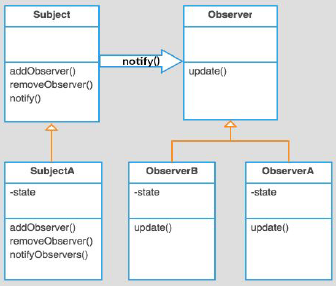
\includegraphics[width=0.4\textwidth]{./observer1}
\end{center}

